\section{Οικογένειες Αθροιστών}
Στο προηγούμενο κεφάλαιο περιγράφηκε ένας απλός σχεδιασμός αθροιστή. Σε αυτή την ενότητα θα γίνει μια περιεκτική παρουσίαση βασικών αρχιτεκτονικών αθροίσματος δυαδικών αριθμών. Σε αυτό το σύνολο ανήκει ο αθροιστής διάδοσης κρατουμένου όπου προαναφέρθηκε, ο αθροιστής παράλειψης και ο αθροιστής επιλογής κρατουμένου καθώς και ο αθροιστής πρόβλεψης κρατουμένου.



\subsection{Διάδοσης Κρατουμένου}
Αθροιστής Διάδοσης Κρατουμένου ή Ripple-Carry Adder (RCA) είναι ο πιο απλός αθροιστής και το σχηματικό του παρουσιάστηκε στην εικόνα \ref{IntegerAdderSchematic}. Παρατηρείται πως για να υπολογιστεί το $sum_1$, δηλαδή το δεύτερο λιγότερο σημαντικό ψηφίο του αθροίσματος, πρέπει πρώτα να υπολογιστεί το $c_{out}$ του προηγούμενου πλήρη αθροιστή, δηλαδή το $c_0$. Αντίστοιχα, για το τρίτο πρέπει να υπολογιστεί πρώτα το $c_0$ έπειτα από τον δεύτερο πλήρη αθροιστή να υπολογιστεί το $c_1$ με είσοδο το $c_0$ του προηγούμενου FA. Επομένως κάθε FA δεν λειτουργεί παράλληλα με τα υπόλοιπα στοιχεία άθροισης, αλλά υπάρχει μια χρονική καθυστέρηση για να λάβει την σωστή είσοδο $c_{in}$. Αποτέλεσμα αυτού είναι πως στην χειρότερη περίπτωση, δηλαδή στην περίπτωση που το $c_{in}$ επηρεάζει άμεσα την τιμή του $c_{out}$ του αθροιστή, υπάρχει γραμμική αύξηση της καθυστέρησης με το μήκος του.
Για παράδειγμα έχοντας έναν δυαδικό αθροιστή 8 ψηφίων και εισάγοντας τους αριθμούς Α = 00000000 και Β = 11111111 και $c_{in}$ = 0 θα πάρουμε έξοδο sum = 11111111 και $c_{out}$ = 0. Κρατώντας όλες τις εισόδους σταθερές και αλλάζοντας μόνο την Α σε 00000001 δηλαδή, το $A_0$=1, τότε το αποτέλεσμα θα είναι sum=00000000 και $c_{out}=1$. 

Η περίπτωση που περιγράφηκε ανήκει στις χειρότερες περιπτώσεις διότι μία αλλαγή στο λιγότερο σημαντικό ψηφίο διαδίδεται στο σημαντικότερο ψηφίο του αθροίσματος καθώς και στο τελικό κρατούμενο εξόδου του αθροιστή, και πρέπει να περάσει από όλα τα ενδιάμεσα στοιχεία άθροισης. Αυτό συνεπάγει και την άθροιση των καθυστερήσεων του κάθε FA στοιχείου για τον υπολογισμό του ολικού χρόνου καθυστέρησης του αθροιστή. Παρόμοια περίπτωση θα καταγραφόταν αν άλλαζε η τιμή του κρατουμένου εισόδου από μηδέν σε ένα, αντί του αριθμού A στο παραπάνω παράδειγμα.

Πρέπει να τονιστεί πως στο σχεδιασμό υλικού προβλέπεται πάντα η χειρότερη περίπτωση χωρίς τον συνυπολογισμό της πιθανότητας εμφάνισης της. Δεν είναι επιτρεπτός ο ορισμός μέσης τιμής καθυστέρησης ενός αθροιστή. Η χρονική τιμή της ταχύτητας ενός κυκλώματος διεξάγεται λαμβάνοντας μετρήσεις στις χείριστες αυτές περιπτώσεις. 




\subsection{Παράλειψης Κρατουμένου}
Για κάθε ψηφίο του αριθμού Α και Β ορίζεται ένα ακόμα στοιχείο. Το σήμα propagate ή p σηματοδοτεί την διάδοση του κρατουμένου εισόδου σε έναν FA. Ορίζεται ένα σήμα p για κάθε ζεύγος δυαδικών ψηφίων των αριθμών εισόδου $(A_i,B_i)$. Η εξίσωση του σήματος αυτού δίνεται:

% , αυτά που παράγουν κρατούμενο ανεξάρτητο του κρατουμένου εισόδου του αντίστοιχου FA και καλούνται generate και αυτά που διαδίδουν κρατούμενο και ονομάζονται propagate. Σημειώνεται πως τα σήματα generate και propagate αναφέρονται στα ζεύγη των δυαδικών ψηφίων των αριθμών εισόδου, δηλαδή $(A_i,B_i)$. Οι εξισώσεις είναι αντίστοιχα:
\begin{equation}
    p_i = A_i \oplus B_i 
\end{equation}

%-----------------
Οι αθροιστές παράλειψής κρατουμένου ή Carry Skip είναι μια υλοποίηση που βελτιώνει την καθυστέρηση διάδοσης κρατουμένου με έναν απλό τρόπο αλλά όχι αρκετά αποτελεσματικό σε σχέση με άλλες αρχιτεκτονικές. Η χείριστη περίπτωση παρουσιάζεται παρομοίως με έναν ripple-carry, δηλαδή, όταν το propagate στοιχείο είναι αληθές για κάθε ζευγάρι ψηφίων $(A_i B_i)$. Όταν όλοι οι όροι propagate είναι αληθείς τότε το κρατούμενο εισόδου προσδιορίζει άμεσα το κρατούμενο εξόδου.
Παίρνοντας κάθε όρο propagate και εισάγοντας τον σε μια n-εισόδων πύλη AND ορίζεται ο όρος select όπου οδηγεί την είσοδο επιλογής ενός πολυπλέκτη 2-σε-1. Η έξοδος του πολυπλέκτη αυτού είναι το κρατούμενο εξόδου $c_{out}$ του αθροιστή, και όταν το select είναι αληθές τότε επιλέγεται το $c_{in}$, αντιθέτως το $c_n$ .
%ΣΗΜΑ 
\begin{equation}
\begin{split}
    p_i &= A_i \oplus B_i \\
    select &= p_0 * p_1 * ... * p_{n-1} \\
    c\_out &= select\ ?\ c\_in\ :\ c_{n-1} % c_n-1 = c_out 
\end{split}
\end{equation}
%ΟΡΙΣΕ ΑΝ ΘΑ ΛΕΣ ΤΟ ΚΡΑΤΟΥΜΕΝΟ ΕΙΣΟΔΟΥ C_0 ‘H C_-1
Η βελτιστοποίηση της χείριστης περίπτωσης επιτυγχάνεται με την χρήση πολλαπλών αθροιστών παράβλεψης κρατουμένου για την δόμηση ενός block-carry-skip αθροιστή. Στην αντίθετη περίπτωση, αν το μέγεθος του αθροιστή είναι μεγάλο (π.χ. 32-bits ή 64-bits) οι καθυστερήσεις είναι σχετικά κοινές με αυτές του ripple-carry. Ο αριθμός των εισόδων της πύλης AND για τον υπολογισμό του select είναι ίσος με το μήκος του αθροιστή με αποτέλεσμα ένας αθροιστής παράλειψής κρατουμένου μεγάλου μήκους να καθίσταται μη πρακτικός. 
%-----------------



\subsection{Επιλογής κρατουμένου}
Ο αθροιστής επιλογής κρατουμένου ή Carry-Sellect Adder υλοποιείται με τον εξής τρόπο :
\begin{itemize}
  \item Δύο αθροιστές ίδιου μήκους εκτελούν τις ίδιες προσθέσεις με την διαφορά πως ο ένας έχει ως κρατούμενο εισόδου 0 και ο άλλος 1.
  \item Το κρατούμενο εισόδου του αθροιστή οδηγεί την είσοδο επιλογής ενός πολυπλέκτη με είσοδο τα αποτελέσματα των δυο αθροιστών που προαναφέρθηκαν.
  \item Ανάλογα με την κατάσταση του κρατουμένου εισόδου επιλέγεται και το σωστό αποτέλεσμα στην έξοδο.
\end{itemize} 
Ομοίως με τον αθροιστή παράβλεψης κρατουμένου, η συγκεκριμένη αρχιτεκτονική έχει πρακτική εφαρμογή όταν εφαρμόζεται σε επιμέρους τμήματα.








\subsection{Πρόβλεψης Κρατουμένου}
Σε αντίθεση με τις προηγούμενες τακτικές βελτίωσης της άθροισης ο Αθροιστής Πρόβλεψης Κρατουμένου ή Carry-Lookahead Adder (CLA) βελτιώνει την ταχύτητα μειώνοντας τον χρόνο υπολογισμού κάθε ενδιάμεσου κρατουμένου καθώς και του τελικού $c_{out}$.
Αυτή η αρχιτεκτονική υλοποιείται με τον παρακάτω τρόπο :
\begin{itemize}
    \item Υπολογίζονται, για κάθε ζεύγος ( $A_i$ , $B_i$ ) δύο σήματα, το ένα αληθεύει όταν το ζεύγος μπορεί να διαδώσει το κρατούμενο που εξάγει το προηγούμενο ζεύγος και το άλλο αληθεύει όταν το παρόν ζευγάρι παράγει κρατούμενο ανεξαρτήτως αν θα έχει κρατούμενο εισόδου ή όχι. Τα σήματα αυτά ονομάζονται propagate ή p και generate ή g, αντίστοιχα.
    \item Συνδυάζοντας αυτά τα σήματα δίνεται η δυνατότητα να προσδιοριστεί ταχύτερα αν ένα τμήμα ζευγών ψηφίων πρόκειται να διαδώσει ή να παράξει ένα κρατούμενο. Κάθε κρατούμενο, ενδιάμεσο ή τελικό, μπορεί να υπολογιστεί ξεχωριστά από την Μονάδα Υπολογισμού Κρατούμενων.
\end{itemize}

Οι εξισώσεις των σημάτων propagate και generate δίνονται:
\begin{equation}
    \begin{split}
        p_i &= a_i + b_i\\
        g_i &= a_ib_i
    \end{split}
\end{equation}

Όταν ισχύει $g_i=1$ τότε γνωστοποιείται πως ο συγκεκριμένος πλήρης αθροιστής παράγει κρατούμενο εξόδου ανεξαρτήτως του κρατουμένου εισόδου. Σε αντίθεση με την συνάρτηση εξόδου του $c_{out}$, του Full-Adder, η συνάρτηση του generate είναι πιο απλή καθώς αποτελείται από μόνο μια πύλη AND, δεν εγγυάται όμως την ύπαρξη κρατούμενο εξόδου. Δηλαδή αν $g_i=1$ τότε και $c\_out_i=1$ χωρίς να ισχύει το αντίθετο. 

Για παράδειγμα σε έναν αθροιστή των τεσσάρων bits χωρίς κρατούμενο εισόδου η διάδοση του κρατουμένου από το πρώτο έως το τελευταίο bit εξαρτάται από την ομάδα διάδοσης κρατουμένου ή Group Propagate (P). Επίσης, η παραγωγή κρατουμένου εξαρτάται από την ομάδα παραγωγής κρατουμένου ή Group Generate (G) των τεσσάρων ζευγών. Για το P είναι εύκολο να βρούμε την συνάρτηση bool του εφόσον το έχουμε συναντήσει και στις παραπάνω ομάδες αθροιστών, αντίθετα το G είναι πιο περίπλοκο. Παρακάτω παρουσιάζονται οι λογικές συναρτήσεις των κρατουμένων αυτού του αθροιστή.
\begin{equation}
    \begin{split}
        c_0 =& g_0 \\
        c_1 =& g_1 + p_1g_0 \\
        c_2 =& g_2 + p_2g_1 + p_2p_1g_0 \\
        c_3 =& g_3 + p_3g_2 + p_3p_2g_1 + p_3p_2p_1g_0 \\
    \end{split}
    \label{eq:cla_carries_4bit}
\end{equation}
Το σήμα $c_3$ είναι το κρατούμενο εξόδου του 4-bit αθροιστή και όπως γίνεται αντιληπτό αντιπροσωπεύει το κρατούμενο που παράγεται από το πρώτο ζεύγος $(Α_0,Β_0)$ έως το τέταρτο $(A_3,B_3)$. Οπότε το $c_3$ είναι και το κρατούμενο που παράγεται από μία ομάδα των τεσσάρων εισόδων και μπορεί να αναπαρασταθεί και ως $G_{3:0}$. Δηλαδή κάθε κρατούμενο αναπαριστάται με την αντίστοιχη ομάδα $c_i = G_{i:0}$. Στην περίπτωση ύπαρξης κρατουμένου εισόδου ισχύει
\begin{equation}
    \begin{split}
        c_i =& G_{i:-1}\\
        c_{in} =& g_{-1} = c_{-1}\\
    \end{split}
\end{equation}
και οι αντίστοιχες εξισώσεις γράφονται
\begin{equation*}
    \begin{split}
        c_0 =& g_0 + p_0c_{-1} \\
        c_1 =& g_1 + p_1g_0 + p_1p_0c_{-1} \\
        c_2 =& g_2 + p_2g_1 + p_2p_1g_0 + p_2p_1p_0c_{-1} \\
        c_3 =& g_3 + p_3g_2 + p_3p_2g_1 + p_3p_2p_1g_0 + p_3p_2p_1p_0c_{-1} \\
    \end{split}
\end{equation*}

Είναι σημαντικό να τονιστεί πως η λογική για τον υπολογισμό των κρατουμένων που μόλις αναφέρθηκε καταλαμβάνει επιπλέον πόρους. Επίσης, κρατούμενα που αφορούν σημαντικότερα ψηφία εισόδου έχουν πολυπλοκότερη λογική, όπως φαίνεται και στην εξίσωση \ref{eq:cla_carries_4bit}. Ο λόγος ύπαρξης των σημάτων Group Propagate P δίνουν την δυνατότητα της τροποποίησης των εξισώσεων των κρατουμένων όπως φαίνεται παρακάτω. 
\begin{equation*}
    c_3 = G_{3:0} = g_3 + p_3g_2 + P_{3:2}g_1 + P_{3:1}g_0 
\end{equation*}
Τα σήματα $G_{i:j}$ και $P_{i:j}$ θα αναλυθούν στο επόμενο κεφάλαιο.

Στην εικόνα \ref{cla_architecture} παρουσιάζεται η βασική αρχιτεκτονική ενός αθροιστή πρόβλεψης κρατουμένου των n δυαδικών ψηφίων. Στο πρώτο επίπεδο υπολογίζονται τα σήματα generate και propagate, στο δεύτερο τμήμα υπολογίζονται τα σήματα Group Generate (κρατούμενα $c_i$) και Group Propagate και στο τρίτο πραγματοποιείται η άθροιση.
\begin{figure}[H]
    \centering
    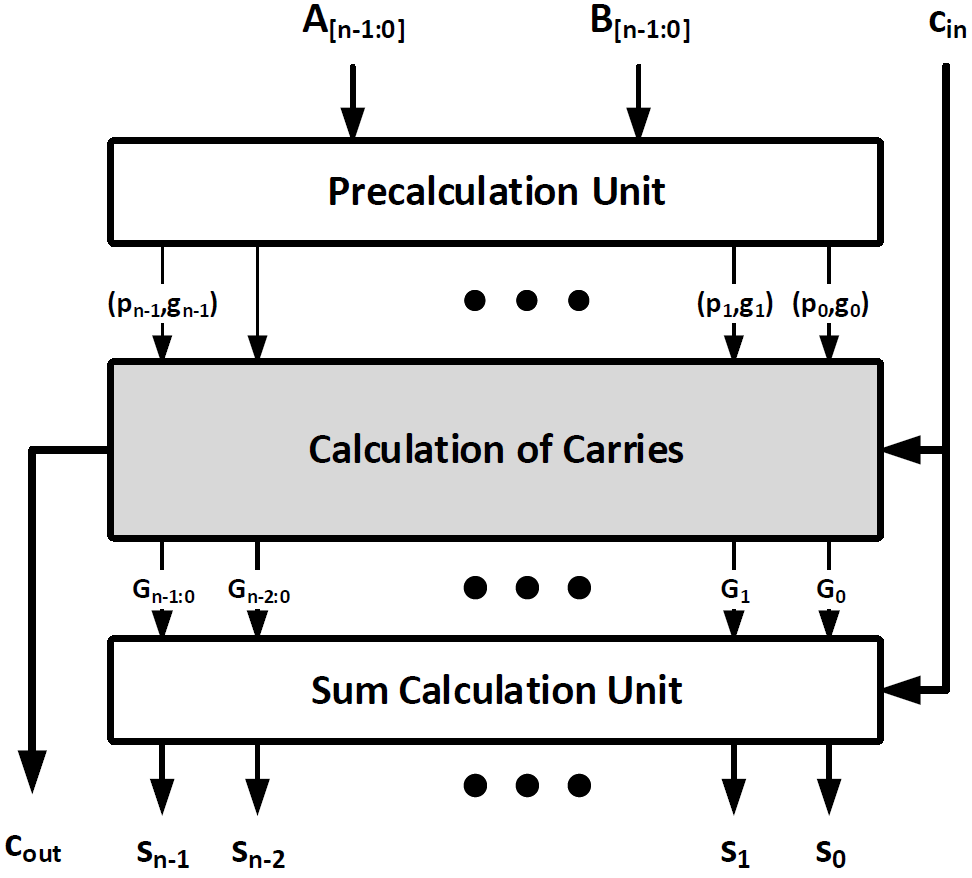
\includegraphics[height=9cm,width=10cm]{Pictures/CLA_Architecture.png}
    \caption{Αρχιτεκτονική αθροιστή πρόβλεψης κρατουμένου}
    \label{cla_architecture}
\end{figure}
 Σημειώνεται στην συγκεκριμένη αρχιτεκτονική το υψηλό λειτουργικό φόρτο καθώς και το εμβαδόν που καταλαμβάνει η μονάδα υπολογισμού των κρατουμένων. Στις επόμενες ενότητες θα εξεταστούν τεχνικές βελτιστοποίησης της μονάδας αυτής.
